\documentclass{article}
\usepackage{graphicx}
\usepackage{color}
\usepackage{comment}
\usepackage{amssymb}
\usepackage{amsthm}

\newtheorem{definition}{Definition}
\newtheorem{property}{Property}
\newtheorem{proposition}{Proposition}
\newtheorem{conjecture}{Conjecture}
\newtheorem{example}{Example}
\newtheorem{notation}{Notation}

%%%%%%%%%%%%%%%%%%%%%%%%%%%%%%%%%%%%%%%%%%%%%%%%%%%%%%%%%%%%%%%%%%%%%

% Algorithms and pseudo code
\usepackage{verbatim}
\usepackage{algorithm}
\usepackage{algorithmicx}
\usepackage{algpseudocode}

% Graphics and display
\usepackage{float}
\usepackage{graphicx}
\usepackage{subfig}
\usepackage{enumerate}
\usepackage{url}
\usepackage{multirow}

% Math symbols and environments
\usepackage{amsmath}
\usepackage{amssymb}
\usepackage{stmaryrd} % \varcurlyvee


\usepackage{calc}%#%
\usepackage{enumitem} %%% used in framed graph

\date{ }
% TikZ

\usepackage{tikz}
\usetikzlibrary{shapes,arrows}
\usetikzlibrary{positioning}
\usetikzlibrary{calc}

\usepackage{tikz-3dplot}

\definecolor{myyellow}{RGB}{255,255,150}
\definecolor{mylavender}{RGB}{125,249,255}
\definecolor{mygreen}{RGB}{144,238,14}
\definecolor{myred}{RGB}{255,0,0}

\newcommand\mytext[3][\scriptsize]{#2\\#1 #3}
\newcommand\mynode[4][]{%
  \node[mynode,#1,text width=\the\dimexpr#2cm] (#3) {\mytext{#3}{#4}}; 
}
\newcommand\mynot[4][]{%
  \node[mynot,#1,text width=\the\dimexpr#2cm] (#3) {\mytext{#3}{#4}}; 
}

\setcounter{secnumdepth}{4}

%%%%%%%%%%%%%%%%
%%%% Macros %%%%
%%%%%%%%%%%%%%%%

%%% Math
\newcommand{\nat}{\mathbb{N}}   % Natural numbers
\newcommand{\rat}{\mathbb{Q}}   % Rational numbers
\newcommand{\real}{\mathbb{R}}  % Real numbers
\newcommand{\runit}{[0, 1]}    % The real unit interval


% = with "hip." on the top, useful for indicating where a hypothesis comes in
\newcommand{\heq}{\stackrel{\text{\fontsize{3pt}{3pt}\selectfont hip.}}{=}}
% = because of the de Morgan laws.
\newcommand{\dmeq}{\stackrel{\text{\tiny{dM}}}{=}}


%%% Sets
\newcommand{\args}{\mathcal{A}} % Set of all arguments
\newcommand{\att}{\mathcal{R}}  % Set of all attacks
\newcommand{\valueset}{L}

%%% Votes on arguments
\newcommand{\varg}{V_{\args}}   % Function giving votes on arguments
\newcommand{\vargpro}[1]{\varg^+\left(#1\right)} % Pro votes on arguments
\newcommand{\vargcon}[1]{\varg^-\left(#1\right)} % Con votes on arguments
\newcommand{\vargtot}[1]{\varg^{max}\left(#1\right)} % Max votes on arguments

%%% Votes on attacks
\newcommand{\vatt}{V_{\att}}   % Function giving votes on attacks
\newcommand{\vattpro}[1]{\vatt^+\left(#1\right)} % Pro votes on attacks
\newcommand{\vattcon}[1]{\vatt^-\left(#1\right)} % Con votes on attacks

%%% Attack relations
% Attackers of a given argument
\newcommand{\attackers}[1]{\att^\text{-}\left(#1\right)} 
% Attackers of a given argument for the alternative framework F'
\newcommand{\altattackers}[1]{\att^{\prime\text{-}}\left(#1\right)}
% Ancestors of given argument according to the attack relation
\newcommand{\ancestors}[1]{\att^*\left(#1\right)} 

%%% Frameworks
\newcommand{\safid}{F}               % A single SAF, given by identifier
\newcommand{\safset}{\mathcal{F}}    % Set of all SAFs

\newcommand{\saf}{\safid = \safbody} % Framework id and respective tuple
\newcommand{\safbody}{\langle \args, \att, \varg, \vatt \rangle} % SAF tuple
\newcommand{\oldsaf}{\safid = \oldsafbody} % Ex Framework id and respective tuple
\newcommand{\oldsafbody}{\langle \args, \att, V \rangle} % old SAF tuple
% Alternative framework, same as \safbody but with ' everywhere ;)
\newcommand{\altsafbody}{\langle \args', \att', \varg', \vatt' \rangle} 

%%% Semantics
\newcommand{\semid}{\mathcal{S}}        % Semantic framework identifier
% Semantic framework tuple
\newcommand{\sembody}{\left\langle \valueset,\SAFand_1, \SAFand_2,\SAFor,\lnot,\tau \right\rangle}
\newcommand{\semdef}{\semid = \sembody}     % Semantic framework id and tuple
\newcommand{\semprod}[1]{\semid^\cdot_{#1}} % Product semantic framework
\newcommand{\semsub}{\semid^\text{-}}       % Subtraction semantic framework
\newcommand{\semmax}{\semid^\text{max}}     % Max semantic framework

\newcommand{\SAFand}{\curlywedge}     % Logical and for SAF equations 
\newcommand{\SAFor}{\curlyvee}        % Logical or for SAF equations
\DeclareMathOperator*{\SAFOr}{\bigcurlyvee} % Big or notation, works as \sum
                             %\varcurlyvee also works, but is smaller
\DeclareMathOperator*{\SAFAnd}{\bigcurlywedge} % Big and notation, works as \sum

\newcommand{\modelset}{\mathcal{M}}   % Set of all models


%#% old commands
\newcommand{\afit}{\textit{AF}}
\newcommand{\af}{\afit = \langle \args, \att \rangle}
\newcommand{\vote}{V}
\newcommand{\sem}{\mathcal{S}}

\newcommand{\ssv}{\mathcal{V}}
\newcommand{\tv}{\mathcal{T}}
\newcommand{\pv}{\mathcal{P}}
\newcommand{\xv}{\mathcal{X}}
\newcommand{\ev}{\mathcal{E}}

\newcommand{\safit}{F}

\newcommand{\tupd}{\curlywedge}
\newcommand{\tatt}{\curlyvee}
\newcommand{\Tatt}{\varcurlyvee}

\newcommand{\argarray}{\{x_1, ..., x_n\}}

\newcommand{\voteset}{\mathcal{V}}
\newcommand{\vpro}{\vote^+}
\newcommand{\vcon}{\vote^-}

%%% Mappings
\newcommand{\mapping}{\Phi}

%%% Macro for framed graph
\newlist{tikzitem}{itemize}{1}
\setlist[tikzitem,1]{label=$\bullet$,nolistsep,leftmargin=*}

%%%%%%%%%%%%%%%%%%%%%%%%%%%%%%%%%%%%%%%%%%%%%%%%%%%%%%%%%%%%%%%%%%%%%
%%%%%%%%%%%%%%%%%%%%%%%%%%%%%%%%%%%%%%%%%%%%%%%%%%%%%%%%%%%%%%%%%%%%%

\begin{document}

\title{Report on ongoing research}

\maketitle

This document is an ongoing work regarding the exercise of realizing some of the abstract ideas and notions we discussed in the \emph{BTC-collaboration} document.




\section{Social Behavior}

Ultimately we strive for our system to satisfy the following property:

\begin{property}
\label{uc}
A user of the system never has an incentive to change his/her vote.
\end{property}

However that's not the case for the time being. Before going into formal definitions, with the following simple example we show that the property does not hold for ESAFs.

%{\color{red}   $\dagger$You may jump to the next line colored in red to skip the example entirely.}

\begin{example}
Assume the fictitious example of a framework with three arguments as depicted in Figure \ref{fig:attacksOnAttacks}. Let $\af$ be an Abstract Argumentation Framework and $\oldsaf$ be a Social Argumentation Framework. Let  $\args = \{a, b, c\}$, $\att = \{(b,a), (c,b)\}$.
Suppose that there is a user utilizing the system, that has five votes to spare in her disposal, and her only objective is increasing argument $a$'s value as much as possible

As can be observed from the values in Table \ref{table:aa}, it makes more sense for the user not to take the straight forward approach and use all of the votes s/he possess on argument $a$. But rather take an in direct approach and use them on argument $c$. Table 1 shows that $a$'s social strength benefits greater from the increase in its attacker's attacker's social support.

%Example of Improved Semantics
% !TEX root = esaf.tex

\begin{figure}[h!]
  \centering
    \subfloat[{}]{
   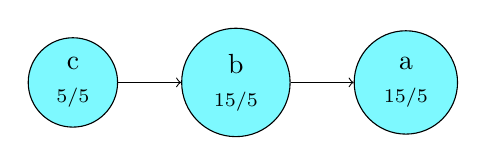
\begin{tikzpicture}[
node distance=0.8cm,
mynode/.style={
  circle,
  draw,
  fill=mylavender,
  text centered}
]
\mynode[]{0.75}{a}{15/5} 
\mynode[left=of a]{0.75}{b}{15/5}
\mynode[left=of b]{0.5}{c}{5/5}  
\draw [->] (b) to [] node [pos=0.4, above, text width=0.9cm]{} (a);
\draw [->] (c) to [] node [pos=0.4, above, text width=0.9cm]{} (b);
\end{tikzpicture}
    \label{subfig:socialsupport}
    
  } \hspace{0.5 cm}
  \subfloat[{}]{
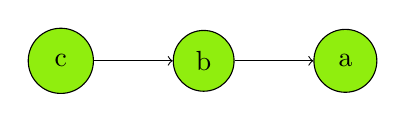
\begin{tikzpicture}[
node distance= 1 cm,
mynode/.style={
  circle,
  draw,
  fill=mygreen,
  text centered}
]
\mynode[]{0.468}{a}{} 
\mynode[left=of a]{0.375}{b}{}
\mynode[left=of b]{0.5}{c}{}  
\draw [->] (b) to [] node [pos=0.4, above, text width=0.9cm]{} (a);
\draw [->] (c) to [] node [pos=0.4, above, text width=0.9cm]{} (b);
\end{tikzpicture}

    \label{subfig:esafmodel}
  }
  
  \caption{ Initial state with votes on arguments(left), Model evaluation under ESAF(right)  }
 \label{fig:attacksOnAttacks}
 
\end{figure}


\begin{figure}[h!]
  \centering
    \subfloat[{}]{
   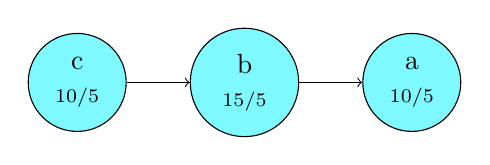
\begin{tikzpicture}[
node distance=0.8cm,
mynode/.style={
  circle,
  draw,
  fill=mylavender,
  text centered}
]
\mynode[]{0.66}{a}{10/5} 
\mynode[left=of a]{0.75}{b}{15/5}
\mynode[left=of b]{0.66}{c}{10/5}  
\draw [->] (b) to [] node [pos=0.4, above, text width=0.9cm]{} (a);
\draw [->] (c) to [] node [pos=0.4, above, text width=0.9cm]{} (b);
\end{tikzpicture}
    \label{subfig:socialsupportAA}
    
  } \hspace{0.5 cm}
  \subfloat[{}]{
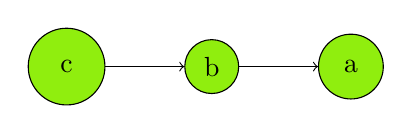
\begin{tikzpicture}[
node distance= 1 cm,
mynode/.style={
  circle,
  draw,
  fill=mygreen,
  text centered}
]
\mynode[]{0.492}{a}{} 
\mynode[left=of a]{0.255}{b}{}
\mynode[left=of b]{0.66}{c}{}  
\draw [->] (b) to [] node [pos=0.4, above, text width=0.9cm]{} (a);
\draw [->] (c) to [] node [pos=0.4, above, text width=0.9cm]{} (b);
\end{tikzpicture}

    \label{subfig:esafmodelAA}
  }
  
  \caption{ Initial state with votes on arguments(left), Model evaluation under ESAF(right)  }
 \label{fig:attacksOnAttacksB}
 
\end{figure}


\renewcommand{\tabcolsep}{0.3cm}
\begin{table}[ht]
  \caption{Model of the Social Abstract Argumentation Framework considering: 1a) social support only; 1b) model under ESAF; 2a) social support only(where 5 positive votes transferred from a to c); 2b) model under ESAF(where 5 positive votes transferred from a to c)\\}
  \centering % used for centering table
\begin{tabular}{c c c c c c} % centered columns (4 columns)
\hline\hline %inserts double horizontal lines
Figure &  Arg. a & Arg. b & Arg. c  \\ [0.7ex] % inserts table 
%heading
\hline % inserts single horizontal line
1a & 0.750 & 0.750 & 0.500 \\ % inserting body of the table
1b & 0,469 & 0,375 & 0,500 \\
2a & 0,667 & 0,750 & 0,667 \\
2b & 0,492 & 0,255 & 0,667 \\ [1ex] % [ex] adds vertical space
\hline %inserts single line
\end{tabular}
\label{table:aa} % is used to refer this table in the text
\end{table}

\end{example}

%{\color{red}   
Thus the example shows in our system, in some settings users indeed have incentive to sway away from their original preferences and vote for other arguments(and/or attack relations).
%} 
This makes it interesting to investigate and figure out potential behavioral patterns of the users.

In the light of this motivation, we first try to construct  the formation. Again we try to define the model as generic as possible, so that later we have the flexibility of tailoring the system for distinctive settings. The model takes some inspiration from other work that mainly dwell in automated task planning and coalition formation.%! ikisi icin de referanslar

\subsection{Social Behavior System}
Let us start by discussing the elements of the system. Firstly several users $\mathcal{U} = {u_1, ..., u_n}$ are involved in the system. 

The system composes several moves  $\mathcal{M} = {m_1, ..., m_n}$ that will be carried out by users. Foreseeable list of moves include  introducing an argument to the system, introducing an attack relation to the system, voting on existing arguments(and/or attack relations).

Each user $u_i \in \mathcal{U}$ is supposed to have a vector of non-negative capabilities $\mathcal{B} = <b_1^i, ..., b_r^i>$. A capability $b_j^i$ represents the capacity of the user $u_i$ regarding the move $m_j$ .  One other way of imagining this vector is a collection of budgets. For instance $m_2$ might stand for the action of voting on an argument, and $b_2^5$ might correspond to the number of votes that user $u_5$ holds that could be used for voting on the existing arguments of the system (Henceforth with respect this modeling $|\mathcal{M}| = |\mathcal{B}^i|$ for any user $u_i \in \mathcal{U}$, but of course for some $b_j^i \in \mathcal{B}^i$, $b_j^i$ might equal to $0$).


Moreover each user $u_i \in \mathcal{U}$ possesses a vector called core, $\mathcal{C}^i = <c_1^i, ..., c_r^i>$. There are multiple possibilities in defining the core. Firstly it could be set of desired entities from the framework, i.e. a subset of the argument set $\mathcal{A}$ (and/or the attack relations set  $\mathcal{R}$). Moreover this set could be substituted by a preference vector. Thus the elements of the core would have a relative hierarchical order between themselves, and this would guide the choices of the user when selecting a move over the rest. 

One more possibility, which a tad more complex is that $\mathcal{C}$ could stand for a desired state of the system, and each $c_i \in \mathcal{C}$ depicts a part of the state. For instance a user might yearn for a state where an argument  $a_i \in \mathcal{A}$ enjoys a social strength higher than 0.7, and an attack relation $(a_m, a_n) \in \mathcal{R}$  to command a social support lower than 0.3,  and an argument $a_j \in \mathcal{A}$ to be attacked by at least five arguments. Such a desired state can be defined via a core with three elements, $\mathcal{C} = <c_1, c_2, c_3>$, where each element correspond to a distinctive one of the three concepts. Again just as stated in the previous discussion, this vector might be defined as preference vector(accompanied by the definition of the necessary operator).

We combine the notions discussed above to construct the formal definition of the envisioned system:

\begin{definition}\textbf{[Social Behavior System]}

A Social Behavior System(SBS) is a triple $<\mathcal{F}, \mathcal{M}, \mathcal{U}>$ such that:

\begin{itemize}
\item $\mathcal{F}$ is an ESAF.
\item  $\mathcal{M} = \{m_1, ..., m_k\}$ is set of moves allowed by the system.
\item $\mathcal{U} = \{u_1, ..., u_l\} $ is a set of users, where $\forall u_i \in \mathcal{U}$ consists of:
\begin{itemize}
\item a vector $\mathcal{C}^i = <c_1^i, ..., c_r^i>$ depicting its core.
\item a vector $\mathcal{B}^i = <b_1^i, ..., b_t^i>$ of its budgets corresponding each move. 
\end{itemize}
\end{itemize}

\end{definition}

\subsection{The concept of Coalition}

In the light of the model, we believe that there are multiple reasons for the users to cooperate under certain settings. 
\begin{itemize}
\item Firstly the shared elements in the cores of the distinct arguments points to an intrinsic motivation for cooperation. 
\item Moreover, recall that we had presented a candidate setting for the notion of core   where the every $c_i \in \mathcal{C}$ corresponds to a desired state of some part of the framework. If a similar approach is adopted,  some arbitrary sub-budget  $b_j^i$ of a user $u_i$ might not prove to be enough for its corresponding element of the core. In such scenarios, we expect the user to look for other users in the hopes of forming a \emph{coalition} to realize such goals which can't be achieved by their own.   
\item Lastly some, negotiation procedures may be defined for the model in order to mimic possible strategic partnerships that may emerge amongst the human users. It may well be plausible for a user to sacrifice the most preferred strategy for the sake of initiating a coalition. 
\end{itemize}

In the light of the listed incentives, we follow with the formal definition of the concept of coalition in our system:

\begin{definition}\textbf{[Coalition]}

Let  $<\mathcal{F}, \mathcal{M}, \mathcal{U}>$ be an SBS, a coalition is a tuple $<\mathcal{K}, \mathcal{G}>$ such that:

\begin{itemize}
\item $K \subseteq U$
\item $\mathcal{G} = \{c_1,..., c_n\} \subseteq \bigcup_{x=1}^{m} C^{x} $, where  $u_i \in K$ for $i \in [1..m]$  % C^1 \cup ... \cup C^m
\item $ \mathcal{K} \Vvdash \mathcal{G}$

\end{itemize}

Where K is the coalition group composed of a set of users, and G is the shared goal which consists of a subset of the union of the cores of the users that belong to the coalition group. $ K \Vvdash G$ denotes that goal $G$ might be realized via K.

\end{definition}

We must note that there are loose ends in the current state of the model, including the formal definitions. Most cases the reason is that, as mentioned above in detail, there are many candidates to be adopted for each concept in the model and the definitions have to be revised for some.

For instance the meaning of the operator $\Vvdash$ from Definition 2 relies on the choice of $\mathcal{C}$. As an example, if we are to follow the first interpretation of $\mathcal{C}$ from Section 1.1 (where roughly, $c_j^i$ corresponds to an entity from the framework, for which the user $u_i$ desires to see an increase in its value), it's probably better to simply drop the operator from the definition. It's hard to talk about \emph{the satisfiability of a goal}, since even an episolon-increase results in a justified cooperation. 

On the other hand if the last approach is adopted from the same section (where briefly, $c_j^i$ a part of a concrete desired state of the frame such as \emph{argument a's social strength being under 0.4}), then the operator indeed serves the intended purpose. This can be seen from its formal definition, which is as follows:

%{\color{red}
\begin{conjecture}\textbf{[Achievement of a unified goal]}

Let  $<\mathcal{F}, \mathcal{M}, \mathcal{U}>$ be an SBS,  $\mathcal{K} \subseteq \mathcal{U}$ and $\mathcal{G} \subseteq \bigcup_{x=1}^{m} \mathcal{C}^{x} $,  for $u_i \in K$, $i \in [1..m]$.

The unified goal $\mathcal{G}$ can be achieved by the group $\mathcal{K}$ of users, denoted by $ \mathcal{K} \Vvdash \mathcal{G}$ , iff $\sum_{u_{i} \in \mathcal{K}} \mathcal{B}^i \geq \sum_{c_{i} \in \mathcal{G}} c_i $ 

%   iff $\forall 1 \leq j \leq r$,    %%amgoud'an ara parca

\end{conjecture}
%}


In plain words, the unified goal is satisfiable if and only if the total budgets of the users in the coalition exceed the numerical value needed to satisfy all the respective cores in the goal. For the sake of simplicity, we suppose $c_i$s are numerical values. Recall that they can be complex sub-states of the framework, so normally these numerical values have to be calculated with a process preceding this check. Moreover we have taken a single-typed budget for all users, where as in sophisticated setting we have to take into consideration of sub-budgets for each move(in other words the definition works adopts a setting of the framework where there is a budget for only one move i.e. solely voting on arguments). 


\subsection{Ongoing work}

As stated earlier, in our system each user aims at maximizing its own utility, or wants to reach its desired state of the framework. When that is not achievable by its own means, each user would have an incentive to seek a coalition with some fellow user(s). 
With this motivation, in this section we have regarded the notion of Social Behavior in our system as a problem of coalition formation that can be defined as a finite set N of users who should achieve a finite set M of cores. 

Ideally, a coalition formation process can be envisioned as a two steps procedure:
\begin{enumerate}
\item Generating the coalition structures. The idea here is to form the coalitions such that
users within a coalition should coordinate to decide on a set of (shared)cores and then achieve those, but
those in different coalitions do not.
\item Discussing these structures between the users in order to select the best ones which
will be adopted.
\end{enumerate}

\subsubsection{Constructing coalition structures}

In the current state of the proposed model, there is no elaborate methodology for constructing coalitions. We may create some simplistic procedures by introducing a few assumptions. For instance we may restrict the cardinality of core set C for each user to one, and state that the users with shared cores form coalitions. This indeed reminds the setting from Prof.Maudet's research, where each user can be easily attained to a party. However this time the number of parties is equal to the number of distinct cores in the system, rather than just two. However there are existing works which may help us in devising a more sophisticated framework in which users have the initiative of choosing the coalition to their liking amongst multiple possibilities. 

Firstly in order to be able to make a choice between the candidate coalitions, users need some type of a preference mechanism. Perhaps this could be achieved by the introduction of a utility function for each user. Given a tuple consisting of a coalition $k_i$ and a user $u_j$,  the value function may return the benefit of attending to $k_i$ for $u_j$.

%{\color{red}
\begin{conjecture}
There exists a function $\mu: \mathcal{U} \times \mathcal{K} \rightarrow \mathcal{P}$, where $(\mathcal{P}, \le)$ is a poset.
\end{conjecture}
%}

So as discussed earlier, we want a function that would give us some idea on how preferable is a certain coalition for a particular user. We envision that this notion would roughly relate to the difference of the profit the user gets via the coalition and the cost of joining the coalition. The profit would perhaps rely on the gain with respect to the cores of the user. And in a similar sense, the cost would depend on the use of budget as a result of the constructed coalition. 

Moreover we envisioned the co-domain of the function to form a poset together with the necessary relation, so that we would have a measure of comparison between distinct coalitions. A total-order or a lattice may prove to be more fruitful, in terms of a more complete comparison measure. On the other hand accomplishing the task of defining such functions with stricter constraints perhaps may turn out to be difficult.   

It's also important to note that with the help of this function, we may formalise Property \ref{uc} which was stated in a highly abstract sense:

%{\color{red}
\begin{conjecture}
$\forall u \in \mathcal{U}$, $\nexists k \in K$ s.t. $\mu(u, k) > \mu(u, \{u\})$ , where $k \neq \{u\}$.
\end{conjecture}
%}

So what the conjecture conveys is that, in the optimal framework for all users there is no coalition setting which would return a higher benefit to the user then acting on its own. Or simpler words, there's no reason at all for cooperating with other users.  


Another interesting notion is \emph{conflicts} between coalitions. Since the budgets are finite values, it might make sense to restrict each user to a single coalition, or a more complex setting could be letting users participate in multiple coalitions as long as they have some remaining budget. However it's thought provoking as it leads to exciting notions like defeasibility. Briefly we may define a \emph{defeat} relation between coalitions, where a coalition defeats another when they share the same cores but the former possess a lower price for formation.

If all these tasks are to be accomplished, then we may upgrade our coalition formation process to a more sophisticated level, consisting of the following four steps:

\begin{enumerate}
\item Constructing  all candidate coalitions.
\item Defining preference and defensibility relations amongst the candidate coalitions.
\item  Hierarchical ordering of the acceptable coalitions (for each user).
\item Actual participation to a certain coalition (for each user).
\end{enumerate}





\section{Vectors meet Pro-arguments}

In this section we try to integrate two distinct research topics that were previously discussed in the \emph{BTC-collaboration} document. We start with a brief recap of the two underlying ideas', possible approaches and their shortcomings.

\subsection{Pro-arguments}

We have been searching for possible methods of including the concept of support into our framework. One candidate extension to the existing framework is the addition of the notion of Pro-arguments, which are envisioned to be structural parts of the arguments they defend rather than stand alone arguments.

Our first take is realizing them as solely additional reasons to make users vote on a particular argument, and leaving them out of the social voting process. This approach does not introduce any additional ways for exploitation of the system (via the users), however it could be seen as merely an enhancement on the GUI side.

Second interpretation is adopting them with the same set of functionalities/privileges as the regular arguments in the framework. However this leaves the system vulnerable against harmful manipulation, i.e. the introduction of fallacious pro-arguments and associating them to existing arguments with strong social support.

 One last realization method of the notion is taking a similar approach to value-based argumentation (as pointed out by Prof.Baroni in his last correspondence). Instead of implementing them as some stripped version of an argument, the idea is mimicking the value functions and making pro-arguments some value promoting relation amongst arguments.  However this method again gives way to the exact same problem as in the second approach.


\subsection{Multi-Dimensional Representation} 

\subsubsection{Preliminaries}

This section will present some useful definitions and notation regarding to (a slightly modified version of) ESAFs. 
\begin{definition}[Extended social argumentation frameworks]
An \emph{extended social argumentation framework} is a 4-tuple $\saf$, where
\begin{itemize}
  \item $\args$ is the set of arguments,
  \item $\att \subseteq \args \times \args$ is a binary attack relation between arguments,
  \item $\varg : \args \to \nat \times \nat \times \nat$ stores the crowd's pro and con votes for each argument together with the maximum number of votes for an argument in the system.
  \item $\vatt : \att \to \nat \times \nat$ stores the crowd's pro and con votes for each attack.
\end{itemize}
\end{definition}

\begin{definition}[Semantic Framework]
\label{def:semfram}
A semantic framework is a 6-tuple \\$\sembody$ where:

\begin{itemize}
  \item $\valueset$ is a totally ordered set with top and bottom elements $\top$, 
$\bot$, containing all possible valuations of an argument. 

  \item $\SAFand_\args,\SAFand_\att:\valueset\times \valueset\rightarrow \valueset$, are two binary algebraic operations used to restrict strengths to given values.
  
  \item $\SAFor:\valueset\times \valueset\rightarrow \valueset$, is a binary algebraic operation on argument valuations used to combine or aggregate valuations and strengths.
  
  \item $\lnot:\valueset\rightarrow \valueset$ is a unary algebraic operation for computing a restricting value corresponding to a given valuation or strength.
  
  \item $\tau : \nat \times \nat \times \nat \to L$ is a function that aggregates positive and negative votes and the maximum number of total votes into a \emph{social support} value.
\end{itemize}
\end{definition}

\begin{notation}
Let $\saf$ be an ESAF, $\sem = \sembody$ a semantic framework and
\begin{itemize}
\item $\attackers{a} \triangleq \{a_i \in \args: (a_i, a) \in \att\}$ be the set of direct attackers of an argument $a \in \args$, 
\item $\vargpro a \triangleq x$ denote the number of positive votes for argument $a$,
\item $\vargcon a \triangleq y$ denote the number of negative votes for argument $a$,
\item $\vargtot a \triangleq z$ denote the number of maximum votes for an argument in the ESAF that argument $a$ belongs to, 
\item $\tau(a) \triangleq \tau(V_{\mathcal{A}}(a))= \tau(x, y, z)$ denote the social support for an argument $a$ via utilizing a vote aggregation function $\tau$, %\tau(\vargpro a, \vargcon a, \vargtot a)
\item $v^r(a) = \frac{\vargpro a}{\vargcon a}$ denote the ratio of positive votes to negative votes for argument $a$,
\item $v^t(a) =\vargpro a + \vargcon a$ denote the total number of votes for argument $a$,
\item $\vattpro{(a, b)} \triangleq m$ denote the number of positive votes for an attack relation between arguments  $a$ and $b$,
\item  $ \vattcon{(a, b)}  \triangleq n$ denote the number of negative votes for an attack relation between arguments  $a$ and $b$,
\item  $\tau((a, b)) \triangleq \tau(\vatt(a,b)) = \tau(m, n)$ denote the social support for an attack relation between arguments  $a$ and $b$ by utilizing a vote aggregation function $\tau$,
\item$$\SAFOr_{x \in R} x \triangleq\left(\left(\left(  x_{1}\SAFor x_{2}\right) \SAFor...\right)\SAFor x_{n}\right)$$ $R=\left\{  x_{1},x_{2},...,x_{n}\right\}$ denote the aggregation of a multiset of elements of $\valueset$. 
\end{itemize}
\end{notation}

\begin{definition}[Model]
\label{def:model}
  Let $\saf$ be a social argumentation framework, $\semdef$ be a semantic framework. A $\semid$-model of $\safid$ is a total mapping $M : \args \rightarrow \valueset$ such that for all $a \in \args$,
  $$\displaystyle M(a) = \tau(a) \SAFand_\args \lnot \SAFOr_{a_i \in \attackers{a}} \left(\tau\left((a_i, a)\right) \SAFand_\att M\left(a_i\right)\right)$$
\end{definition}



\subsubsection{Properties and Propositions}

Again in the previous document, we had discussed the fact that even though we have functions for unifying the social such as the one depicted in Definition 4, accompanied by a set of desired properties(P1, P2, P3), there is substantial room for improvement. 

%% vector ozet


\begin{definition}
\label{def:voteAgg}
[Enhanced Vote Aggregation]
\\ An enhanced vote aggregation function is any function
$\tau:
\mathbb{N} \times \mathbb{N} \times \mathbb{N}
\rightarrow\lbrack0,1]$ such that $v_{max}\geq0$
\[
\tau\left(  v^{+},v^{-}, v_{max}\right)  =\left\{
\begin{array}
[c]{lll}
0 &  & v_{max}=0\\
\frac{v^{+}}{v^{+}+v^{-}+\frac{1}{v_{max}}} &  & \text{otherwise}
\end{array}
\right.
\]

%where $v_{max}$ stands for the maximum number of votes for an argument in the system.
\end{definition}

{\color{red}
\begin{property}
\label{P1} [Perfect argument freeness] \\
Let $\saf$ be an ESAF and $\semdef$ a semantic framework. A vote aggregation function $\tau : \nat \times \nat \times \nat \to L$ is said to be "perfect argument free" if
\begin{center}
$\forall a \in \mathcal{A}$, $\tau \left(a\right) < 1$. %$\tau \left( v^{+},v^{-}, v_{max}\right) \neq 1$
\end{center}
\end{property}
}

The gist of the property can be captured in a verbal context with the following sentence: \emph{No argument enjoys perfect Social Support.}  \\

\begin{proposition}
Enhanced Vote Aggregation function enjoys Property \ref{P1}.
\end{proposition}

\begin{proof} Trivial.
\\
Suppose an arbitrary $a \in \args$ of an extended social argumentation framework $\mathcal{F}$ with some well-behaved semantics $\mathcal{S}$:\\
If $v^+ = 0$ then $\tau(a) = \tau(v^{+}, v^{-}, v_{max}) = 0 \le 1$. \\
Else if $v^+ \neq 0$, then $v_{max} \neq 0$ and since $v_{max} \in \mathcal{Z}^+$, then $\frac{1}{v_{max}} > 0.$ Since denominator equals to the addition of the numerator and some $r \in {R}^+ $, denominator is bigger than the numerator and thus \\
$ \frac{v^{+}}{v^{+}+v^{-}+\frac{1}{v_{max}}} = \tau(v^{+}, v^{-}, v_{max}) \le 1$.

\end{proof}

{\color{red}
\begin{property}
\label{P2}[Precedence of the vote ratio]\\
Let $\saf$ be an ESAF and $\semdef$ a semantic framework.  For $a_1, a_2 \in \args$, a vote aggregation function $\tau : \nat \times \nat \times \nat \to L$ is said to be "vote ratio precedent" if
\begin{center}
 $\left( v^{r}(a_{1}) \ge v^{r}(a_{2}) \right) \implies \left( \tau(a_1) \ge \tau(a_2) \right)$. 
\end{center}

\end{property}
}

The gist of the property can be captured in a verbal context with the following sentence: \emph{If the value of the ratio of positive votes to the total amount of votes is higher for an argument $a$ than an argument $b$; $a$'s social support value exceeds the social support of $b$.}  \\

\begin{conjecture}
Vote Aggregation function enjoys Property \ref{P2}.
\end{conjecture}

\begin{proof}  [Sketch of proof] It should suffice to show that:
\\
For two arbitrary tuples $(v^+_1, v^-_1)$ and $(v^+_2, v^-_2)$, if $\frac{v^+_1} {v^-_1} \ge \frac{v^+_2} {v^-_2}$ then $\tau(v^+_1, v^-_1, v_{max}) \ge \tau(v^+_2, v^-_2, v_{max})$. 

\end{proof}


As an example for  $(v^+_1, v^-_1) = (10,0)$ and $(v^+_2, v^-_2) = (999,1)$, $v_{max} = 1000$ and $\tau(v^+_1, v^-_1, v_{max}) = 0.9999$ and  $\tau(v^+_2, v^-_2, v_{max}) = 0.9989$.

{\color{red}
\begin{property}
\label{P3}[Precedence of the total number of votes] \\
Let $\saf$ be an ESAF and $\semdef$ a semantic framework.  For $a_1, a_2 \in \args$, a vote aggregation function $\tau : \nat \times \nat \times \nat \to L$ is said to be "total votes precedent" if
\begin{center}
 $\left( \left(v^{r}(a_{1}) = v^{r}(a_{2}) \right) \land  \left( v^{t}(a_{1}) \ge ( v^{t}(a_{2}) \right) \right) \implies \left( \tau(a_1) \ge \tau(a_2) \right)$. 
\end{center}
\end{property}
}

The gist of the property can be captured in a verbal context with the following sentence: \emph{When the ratios are equal, the function should return a higher social support value for the one with the higher number of total votes.}  \\

\begin{conjecture}
Enhanced Vote Aggregation function enjoys Property \ref{P3}.
\end{conjecture}

\begin{proof}  [Sketch of proof] It should suffice to show that:
\\
 For two tuples $(v^+_1, v^-_1)$ and $(v^+_2, v^-_2)$, if $\frac{v^+_1} {v^-_1} = \frac{v^+_2} {v^-_2}$ and $( v^+_1 + v^-_1) \ge ( v^+_2 + v^-_2)$ then $\tau(v^+_1, v^-_1, v_{max}) \ge \tau(v^+_2, v^-_2, v_{max})$.
\end{proof}


As an example for $(v^+_1, v^-_1) = (45,5)$ and $(v^+_2, v^-_2) = (9,1)$, $v_{max} = 50$ and $\tau(v^+_1, v^-_1, v_{max}) = 0.8996$ and  $\tau(v^+_2, v^-_2, v_{max}) = 0.8982$




\vspace{10 mm}

However firstly, the existing function's result does not reflect the total number of votes casted on a particular argument to a decent extent. Moreover since the function boils all the inputs to a single value prior to the model evaluation, we don't have much flexibility in the upcoming stages of the computation.

With ESAFs, when two distinct arguments have the same ratio of positive and negative votes, even if they differ immensely with respect to the total number of votes they've received, this fact is not reflected in their model evaluation values. 

We may capture the idea with the following property:

%{\color{red}
\begin{property}
\label{pro:dim}
"For two arguments sharing the same ratio of positive and negative votes and the same set of attackers, if the total number of votes differ from each other, so should the model evaluations."\\
Let $\saf$ be an extended social argumentation framework, $\semdef$ a well behaved semantics and $\mathcal{\mathcal{M}}^F_{\mathcal{S}}$ the set of all $\mathcal{S}$-models of $\mathcal{F}$.  For $a_1, a_2 \in \args$, where $a_1 = (v^+_1, v^-_1)$,  $a_2 = (v^+_2, v^-_2)$, and  $\attackers {a_1} = \attackers {a_2}$, and $v^+_1 \neq 0$, $v^+_2 \neq 0$,
\begin{center}
$\forall M \in \mathcal{\mathcal{M}}^F_{\mathcal{S}},  \left( \left( \frac{v^+_1} {v^-_1} = \frac{v^+_2} {v^-_2} \right) \land  \left(( v^+_1 + v^-_1) \neq ( v^+_2 + v^-_2) \right) \right) \implies \left( M(v^+_1, v^-_1) \neq M(v^+_2, v^-_2) \right)$.
\end{center}

\end{property}
%}

We show that the original proposal does not possess to this property.

%{\color{red}
\begin{proposition}
ESAFs do not satisfy Property \ref{pro:dim}.
\end{proposition}

\begin{proof}
It's enough to show a counter-example. Suppose  two arguments $a_1, a_2 \in \args$ of an extended social argumentation framework $\mathcal{F}$ with some well-behaved semantics $\mathcal{S}$ such that
\begin{itemize}
\item the arguments have some positive votes:  $v^+_1 \neq 0$, $v^+_2 \neq 0$  ,
\item the arguments are unattacked:      $\attackers {a _1}= \emptyset$, $\attackers {a_2}= \emptyset$
\item and the ratios of positive to negative votes are the same:  $ \left( \frac{v^+_1} {v^-_1} = \frac{v^+_2} {v^-_2} \right)$ ,
\item and the total number of casted votes are distinct:   $\left(( v^+_1 + v^-_1) \neq ( v^+_2 + v^-_2) \right)$ ,
\item however the model evaluations are the same: $M(v^+_1, v^-_1) = M(v^+_2, v^-_2)$. \\
\end{itemize}


Since $(\frac{v_1^+}{v_1^-} = \frac{v_2^+}{v_2^-})$, $\exists r \in \mathcal{R}^+$ s.t. $v_1^+ \cdot r = v_2^+$ and $v_1^- \cdot r = v_2^-$.

 \begin{align*}
    \tau(a_1) &= \frac{v^{+}_1}{v^{+}_1+v^{-}_1+\varepsilon} \cong  \frac{v^{+}_1}{v^{+}_1+v^{-}_1} \\%\text{, which by commutativity}\\
         &=  \frac{v^{+}_1 \cdot r}{(v^{+}_1+v^{-}_1) \cdot r} =  \frac{v^{+}_1 \cdot r}{v^{+}_1 \cdot r + v^{-}_1 \cdot r  } \\
         &= \frac{v^{+}_2}{v^{+}_2+v^{-}_2} \cong  \frac{v^{+}_2}{v^{+}_2+v^{-}_2+\varepsilon} \\
         &= \tau(a_2)
  \end{align*}

We know that in ESAFS for any unattacked argument $a$, $\tau(a) = M(a)$ for $M \in \mathcal{M}^F_{\mathcal{S}}$. Thus
\begin{center}
$M(a_1) = \tau(a_1) = \tau(a_2) = M(a_2).$\\
CONTRADICTION!
\end{center}

\end{proof}
%}

A multi-dimensional vector representation of an argument lets one tailor operations for each distinct dimension, and then merge them at a phase up to the designer's liking. Since ESAFs assume is no restriction on the labeling set where arguments take their values from, arguments can be maintained as vectors all the way including the model evaluation phase, and the final result might be displayed by some GUI choice depicting all arguments' vector representations. 


\subsection{Marrying the two concepts}
\label{sec:marry}

In the light of the aforementioned motivations, we try to propose a candidate vector representation. 

The first step is defining the dimensions. In one of the earlier \emph{BTC-collaboration} document's iterations we had briefly discussed the possible pitfalls of choosing hybrid dimensions - dimensions consisting of multiple variables, and some of these variables appearing in more than one dimension. This problem is inspected in more detail in the last subsection.

The obvious candidates are the positive and the negative number of votes an argument has received. Moreover in Section 2.1 we have motivated the extension of our system via pro-arguments, but the discussed methods all had their share bit of shortcomings. Here we try to incorporate them to the system by defining them as the third dimension.

Firstly we extend the framework as follows:

\begin{definition}[Tridimensional Social argumentation frameworks]
A tridimensional social argumentation framework is a 6-tuple $\langle \args, \mathcal{P}, \att, \mathcal{M}_P,  \varg, \mathcal{V}_P \rangle$, where
\begin{itemize}
  \item $\mathcal{A}$ is the set of arguments,
  \item  $\mathcal{P}$ is the set of pro-arguments,
  %\item $\args \subseteq \mathcal{B} \times 2^{\mathcal{P}}$  is the set of arguments,
  \item $\att \subseteq \args \times \args$ is a binary attack relation between arguments,
 \item $\mathcal{M}_P: 2^{\mathcal{P}} \to \args$ is a mapping from a set of pro-argument to an argument
  \item $\varg : \args \to \nat \times \nat$ stores the crowd's pro and con votes for each argument.
%  \item $\vatt : \att \to \nat \times \nat$ stores the crowd's pro and con votes for each attack.
\item $\mathcal{V}_P : \mathcal{P} \to \nat \times \nat$ stores the crowd's pro and con votes for each pro-argument.
%\item Rest of the notions follow the ESAF definition given in \cite{eml2013esaf}. 

(We omit the social voting on attack relations for simplicity.)
\end{itemize}
\end{definition}

Moreover assume we have an aggregation function that given a set of pro-arguments, return a reel value via aggregating each pro-argument's positive and negative votes by some method:  $\psi: 2^{\mathcal{P}} \to \nat$

We may also chose to normalise the pro and con votes of an argument for determining the associated dimension values with some function $\tau: \nat \to  \nat$

Then we may represent each argument $a_i \in \args$ as a vector:

 $\vec{a_i} = < \tau(v_{i}^+),  \tau(v_{i}^-), \psi(\mathcal{M}_{p}^{-}(a_{i}))>$.


Under this topic, current efforts are invested in finding a concrete complete framework utilizing vector operations and leaving the end result (after model evaluation) in vector form.

A very simplistic method $\tau$ can be defined for pro and con votes of the argument as such as:
\begin{center}
$\tau(x) = \frac{x}{v_{max} + \epsilon}$, where $v_{max}$ stands for the maximum number of total votes for an argument in the system.
\end{center}

Thus the values are restricted between the interval of $[0,1] \in \mathbb{R}$, no argument can take the perfect value(i.e. 1) for either dimension(as a result of epsilon addition), and only an argument possessing solely positive votes and  the maximum number of votes in the system would enjoy near perfect value . 

%\subsubsection{Example comparing 2D representation against the framework of TAFA}

\begin{comment}

\begin{tikzpicture}%[line/.style={&gt;=latex}]
\coordinate (V1) at (1, 1.3);
\coordinate (V2) at (-1.6, 0.4);
\coordinate (V3) at ($(V1) + (V2)$);
\coordinate (V4) at ($1.4*(V1)$);
 
\draw[step=10pt, color=black!10] (-2, -1) grid (2, 2);
\draw[&lt;-&gt;, line] (-2, 0) -- node [below, very near end] {$x$} (2, 0);
\draw[&lt;-&gt;, line] (0, -1) -- node [right, very near start] {$y$} (0, 2);
\draw[-&gt;, line, color=orange, thick] (0, 0) -- node [right=2pt, near end] {$\vec{u}$} (V4);
\draw[-&gt;, line, color=blue, thick, densely dashed] (0, 0) -- node [right=2pt] {$\vec{v}$} (V1);
\draw[-&gt;, line, color=red, thick] (0, 0) -- node [above] {$\vec{w}$} (V2);
\draw[-&gt;, line, color=red, densely dotted] (V1) -- +(V2);
\draw[-&gt;, line, color=blue, densely dotted] (V2) -- +(V1);
\draw[-&gt;, line, color=green!70!black, thick] (0, 0) -- node [left] {$\vec{z}$} (V3);
\end{tikzpicture}

\end{comment}

%\subsubsection{An exercise of a concrete semantics}

On the other hand, the following function could perhaps be a suitable choice for the sake of aggregating pro-arguments:
\\
\begin{center}
$ \psi(\{p_1,...,p_n\})  =   \frac { \sum\limits_{i=1}^n \frac{v^{+}_i}{v^{+}_i+v^{-}_i+\frac{1}{(v^{+}_i+v^{-}_i+\frac{1}{v_{max}})}} } {n} $,\\
\end{center}

where $p_{i} \in \mathcal{P}$ for $i \in [1..n]$, $p_i \doteq (v^{+}_{i}, v^{-}_{i})$ with small abuse of notation.
\\ \\
So as can be observed the function first evaluates a single value for each pro-argument's positive and negative votes via utilizing function \ref{def:voteAgg} which contained multiple desirable properties. Then process simply follows taking the average of these numbers.

So in the envisioned system one dimension of the vector representation of the arguments is saved for the value obtained by pro-arguments. We believe that this value should be  acquired in a fair way from the complete set of pro-arguments, and so none of the pro-arguments should dominate the values of the rest by itself. This idea maybe captured with the following property:

%{\color{red}
\begin{property}
\label{proAut}
"No single pro-argument should be an authority by itself." \\
Let $\mathcal{F} = \langle \args, \mathcal{P}, \att, \mathcal{M}_P,  \varg, \mathcal{V}_P \rangle$ be a tridimensional social argumentation framework and $\mathcal{S}=\left\langle L,\tau,\psi, \curlywedge,\curlyvee,\lnot\right\rangle $ a well behaved semantics. % a well-behaved semantic framework$
\begin{center}
$\nexists p \in \mathcal{P}$ s.t. $\forall S \subseteq \mathcal{P}$, $\psi(S \cup \{p\} ) = \psi(\{p\})$.
\end{center}

\end{property}

\begin{proposition}
Choice of T-norms(and respective co-norms) as semantics violate Property \ref{proAut}.
\end{proposition}

\begin{proof}
For the proof it suffices to show that any t-conorm $\bot$ has a zero-element.

  \begin{align*}
    \bot(a,b) &= 1 - \top(1-a, 1-b)   \hspace{10 mm} \text{, Definition of t-conorm} \\
    \bot(a,1) &= 1 - \top(1-a, 1-1) \\
	 &= 1 - \top(1-a, 0)  \hspace{16 mm} \text{, $\top$(x, 0) = 0}\\
	 &= 1 - 0\\
         &= 1
  \end{align*}

\end{proof}
%}

Thus as mentioned above, since for any t-conorm there is a zero element(specifically 1), aforementioned property does not hold. If t-conorms where utilized for the aggregation of pro-arguments, one pro-argument with perfect score, or in other words a pro-argument free of negative votes could surpass the rest.



\subsubsection{A complete example using 3D representation with pro-arguments}

%\begin{figure}
\begin{tikzpicture}[
mynode/.style={
  circle,
  draw,
  fill=yellow,
  minimum size=1cm,
  text width=2.5cm,
  align=center
  },
frame/.style={
  draw=cyan,
  line width=3pt,
  text width=5cm,
  rounded corners
  },
ar/.style={
  ->,
  >=latex
  }    
]
\node[mynode] (a) { {\color{brown} (a) } \\ Portugal has the best team but won't win the WC. \\ {\color{red} (61/35)} };
\node[mynode,below right=2cm and 6cm of a]  (c) { {\color{brown} (c) } \\Portugal will win the WC. \\ {\color{red} (85/16)} };  
\node[mynode,below left=2cm and 6cm of c]  (b) { {\color{brown} (b) } \\Brazil has the best team thus will win the WC. \\ {\color{red} (56/21)} };  

\node[frame,anchor=north west] at (a.-80) 
  {%
  \begin{tikzitem} 
  \item B.Alves receieves too many cards. {\color{red} 15/10}
  \item H.Almeida\&R.Meireles are injury prone.  {\color{red} 23/8}
  \item M.Fernandes isn't included in the squad.  {\color{red} 8/8}
  \item Unreliable technical staff.  {\color{red} 5/25}
  \end{tikzitem}%
  };
\node[frame,anchor=north west] at (b.-90) 
%\node[frame,anchor=south west] at (b.90) 
  {%
  \begin{tikzitem} 
  \item Hosts the cup.  {\color{red} 30/7}
  \item Strikers are on good form.  {\color{red} 14/9}
  \item 5 times cup-holder.  {\color{red} 33/4}
  \end{tikzitem}% 
  };
\node[frame,anchor= north west] at (c.-90)
  {%
  \begin{tikzitem} 
  \item Has the best player on the world.  {\color{red} 41/13}
  \item Proven defensive line.  {\color{red} 22/5}
  \item Fast wingers.  {\color{red} 17/6}
  \end{tikzitem}%
  };

\draw[ar] (a) to[bend left] (c);  
\draw[ar] (b) to[bend right] (c);  
\draw[ar] (a) to[bend right] (b);  
\draw[ar] (b) to[] (a);  
\end{tikzpicture}
%\caption{}
%\end{figure}




%%%%%%%%%% 3D arg A %%%%%%%%%%

\begin{figure}[h!]
  \centering
    \subfloat[{}]{

\tdplotsetmaincoords{60}{120} 
\begin{tikzpicture} [scale=2.5, tdplot_main_coords, axis/.style={->,blue,thick}, 
vector/.style={-stealth,red,very thick}, 
vector guide/.style={dashed,red,thick}]

%standard tikz coordinate definition using x, y, z coords
\coordinate (O) at (0,0,0);

%tikz-3dplot coordinate definition using x, y, z coords

\pgfmathsetmacro{\ax}{0.603}
\pgfmathsetmacro{\ay}{0.346}
\pgfmathsetmacro{\az}{0.502}

\coordinate (P) at (\ax,\ay,\az);

%draw axes
\draw[axis] (0,0,0) -- (1,0,0) node[anchor=north east]{$x$};
\draw[axis] (0,0,0) -- (0,1,0) node[anchor=north west]{$y$};
\draw[axis] (0,0,0) -- (0,0,1) node[anchor=south]{$z$};

%draw a vector from O to P
\draw[vector] (O) -- (P) node[anchor=north west]{$\vec{a}$};

%draw guide lines to components
\draw[vector guide]         (O) -- (\ax,\ay,0);
\draw[vector guide] (\ax,\ay,0) -- (P);
\draw[vector guide]         (P) -- (0,0,\az);
\draw[vector guide] (\ax,\ay,0) -- (0,\ay,0);
\draw[vector guide] (\ax,\ay,0) -- (0,\ay,0);
\draw[vector guide] (\ax,\ay,0) -- (\ax,0,0);
\node[tdplot_main_coords,anchor=east]
at (\ax,0,0){(\ax, 0, 0)};
\node[tdplot_main_coords,anchor=west]
at (0,\ay,0){(0, \ay, 0)};
\node[tdplot_main_coords,anchor=south]
at (0,0,\az){(0, 0, \az)};
\end{tikzpicture}


 } \hspace{-1 cm}
  \subfloat[{}]{

\tdplotsetmaincoords{60}{120} 
\begin{tikzpicture} [scale=2.5, tdplot_main_coords, axis/.style={->,blue,thick}, 
vector/.style={-stealth,red,very thick}, 
vector guide/.style={dashed,red,thick}]

%standard tikz coordinate definition using x, y, z coords
\coordinate (O) at (0,0,0);

%tikz-3dplot coordinate definition using x, y, z coords

\pgfmathsetmacro{\ax}{0.403}
\pgfmathsetmacro{\ay}{0.295}
\pgfmathsetmacro{\az}{0.220}

\coordinate (P) at (\ax,\ay,\az);

%draw axes
\draw[axis] (0,0,0) -- (1,0,0) node[anchor=north east]{$x$};
\draw[axis] (0,0,0) -- (0,1,0) node[anchor=north west]{$y$};
\draw[axis] (0,0,0) -- (0,0,1) node[anchor=south]{$z$};

%draw a vector from O to P
\draw[vector] (O) -- (P) node[anchor=north west]{$\vec{a}$};

%draw guide lines to components
\draw[vector guide]         (O) -- (\ax,\ay,0);
\draw[vector guide] (\ax,\ay,0) -- (P);
\draw[vector guide]         (P) -- (0,0,\az);
\draw[vector guide] (\ax,\ay,0) -- (0,\ay,0);
\draw[vector guide] (\ax,\ay,0) -- (0,\ay,0);
\draw[vector guide] (\ax,\ay,0) -- (\ax,0,0);
\node[tdplot_main_coords,anchor=east]
at (\ax,0,0){(\ax, 0, 0)};
\node[tdplot_main_coords,anchor=west]
at (0,\ay,0){(0, \ay, 0)};
\node[tdplot_main_coords,anchor=south]
at (0,0,\az){(0, 0, \az)};
\end{tikzpicture}
}
  \caption{Social support values  (left), and social strength values of the dimensions for argument $a$ (right)}  
\end{figure}


%%%%%%%%%% 3D arg B %%%%%%%%%%

\begin{figure}[h!]
  \centering
    \subfloat[{}]{

\tdplotsetmaincoords{60}{120} 
\begin{tikzpicture} [scale=2.5, tdplot_main_coords, axis/.style={->,blue,thick}, 
vector/.style={-stealth,red,very thick}, 
vector guide/.style={dashed,red,thick}]

%standard tikz coordinate definition using x, y, z coords
\coordinate (O) at (0,0,0);

%tikz-3dplot coordinate definition using x, y, z coords

\pgfmathsetmacro{\ax}{0.554}
\pgfmathsetmacro{\ay}{0.207}
\pgfmathsetmacro{\az}{0.770}

\coordinate (P) at (\ax,\ay,\az);

%draw axes
\draw[axis] (0,0,0) -- (1,0,0) node[anchor=north east]{$x$};
\draw[axis] (0,0,0) -- (0,1,0) node[anchor=north west]{$y$};
\draw[axis] (0,0,0) -- (0,0,1) node[anchor=south]{$z$};

%draw a vector from O to P
\draw[vector] (O) -- (P) node[anchor=north west]{$\vec{b}$};

%draw guide lines to components
\draw[vector guide]         (O) -- (\ax,\ay,0);
\draw[vector guide] (\ax,\ay,0) -- (P);
\draw[vector guide]         (P) -- (0,0,\az);
\draw[vector guide] (\ax,\ay,0) -- (0,\ay,0);
\draw[vector guide] (\ax,\ay,0) -- (0,\ay,0);
\draw[vector guide] (\ax,\ay,0) -- (\ax,0,0);
\node[tdplot_main_coords,anchor=east]
at (\ax,0,0){(\ax, 0, 0)};
\node[tdplot_main_coords,anchor=west]
at (0,\ay,0){(0, \ay, 0)};
\node[tdplot_main_coords,anchor=south]
at (0,0,\az){(0, 0, \az)};
\end{tikzpicture}


 } \hspace{-1 cm}
  \subfloat[{}]{

\tdplotsetmaincoords{60}{120} 
\begin{tikzpicture} [scale=2.5, tdplot_main_coords, axis/.style={->,blue,thick}, 
vector/.style={-stealth,red,very thick}, 
vector guide/.style={dashed,red,thick}]

%standard tikz coordinate definition using x, y, z coords
\coordinate (O) at (0,0,0);

%tikz-3dplot coordinate definition using x, y, z coords

\pgfmathsetmacro{\ax}{0.330}
\pgfmathsetmacro{\ay}{0.145}
\pgfmathsetmacro{\az}{0.561}

\coordinate (P) at (\ax,\ay,\az);

%draw axes
\draw[axis] (0,0,0) -- (1,0,0) node[anchor=north east]{$x$};
\draw[axis] (0,0,0) -- (0,1,0) node[anchor=north west]{$y$};
\draw[axis] (0,0,0) -- (0,0,1) node[anchor=south]{$z$};

%draw a vector from O to P
\draw[vector] (O) -- (P) node[anchor=north west]{$\vec{b}$};

%draw guide lines to components
\draw[vector guide]         (O) -- (\ax,\ay,0);
\draw[vector guide] (\ax,\ay,0) -- (P);
\draw[vector guide]         (P) -- (0,0,\az);
\draw[vector guide] (\ax,\ay,0) -- (0,\ay,0);
\draw[vector guide] (\ax,\ay,0) -- (0,\ay,0);
\draw[vector guide] (\ax,\ay,0) -- (\ax,0,0);
\node[tdplot_main_coords,anchor=east]
at (\ax,0,0){(\ax, 0, 0)};
\node[tdplot_main_coords,anchor=west]
at (0,\ay,0){(0, \ay, 0)};
\node[tdplot_main_coords,anchor=south]
at (0,0,\az){(0, 0, \az)};
\end{tikzpicture}
}
  \caption{Social support values  (left), and social strength values of the dimensions for argument $b$ (right)}  
\end{figure}


%%%%%%%%%% 3D arg C%%%%%%%%%%

\begin{figure}[h!]
  \centering
    \subfloat[{}]{

\tdplotsetmaincoords{60}{120} 
\begin{tikzpicture} [scale=2.5, tdplot_main_coords, axis/.style={->,blue,thick}, 
vector/.style={-stealth,red,very thick}, 
vector guide/.style={dashed,red,thick}]

%standard tikz coordinate definition using x, y, z coords
\coordinate (O) at (0,0,0);

%tikz-3dplot coordinate definition using x, y, z coords

\pgfmathsetmacro{\ax}{0.841}
\pgfmathsetmacro{\ay}{0.158}
\pgfmathsetmacro{\az}{0.746}

\coordinate (P) at (\ax,\ay,\az);

%draw axes
\draw[axis] (0,0,0) -- (1,0,0) node[anchor=north east]{$x$};
\draw[axis] (0,0,0) -- (0,1,0) node[anchor=north west]{$y$};
\draw[axis] (0,0,0) -- (0,0,1) node[anchor=south]{$z$};

%draw a vector from O to P
\draw[vector] (O) -- (P) node[anchor=north west]{$\vec{c}$};

%draw guide lines to components
\draw[vector guide]         (O) -- (\ax,\ay,0);
\draw[vector guide] (\ax,\ay,0) -- (P);
\draw[vector guide]         (P) -- (0,0,\az);
\draw[vector guide] (\ax,\ay,0) -- (0,\ay,0);
\draw[vector guide] (\ax,\ay,0) -- (0,\ay,0);
\draw[vector guide] (\ax,\ay,0) -- (\ax,0,0);
\node[tdplot_main_coords,anchor=east]
at (\ax,0,0){(\ax, 0, 0)};
\node[tdplot_main_coords,anchor=west]
at (0,\ay,0){(0, \ay, 0)};
\node[tdplot_main_coords,anchor=south]
at (0,0,\az){(0, 0, \az)};
\end{tikzpicture}


 } \hspace{-1.2 cm}
  \subfloat[{}]{

\tdplotsetmaincoords{60}{120} 
\begin{tikzpicture} [scale=2.5, tdplot_main_coords, axis/.style={->,blue,thick}, 
vector/.style={-stealth,red,very thick}, 
vector guide/.style={dashed,red,thick}]

%standard tikz coordinate definition using x, y, z coords
\coordinate (O) at (0,0,0);

%tikz-3dplot coordinate definition using x, y, z coords

\pgfmathsetmacro{\ax}{0.335}
\pgfmathsetmacro{\ay}{0.095}
\pgfmathsetmacro{\az}{0.255}

\coordinate (P) at (\ax,\ay,\az);

%draw axes
\draw[axis] (0,0,0) -- (1,0,0) node[anchor=north east]{$x$};
\draw[axis] (0,0,0) -- (0,1,0) node[anchor=north west]{$y$};
\draw[axis] (0,0,0) -- (0,0,1) node[anchor=south]{$z$};

%draw a vector from O to P
\draw[vector] (O) -- (P) node[anchor=north west]{$\vec{c}$};

%draw guide lines to components
\draw[vector guide]         (O) -- (\ax,\ay,0);
\draw[vector guide] (\ax,\ay,0) -- (P);
\draw[vector guide]         (P) -- (0,0,\az);
\draw[vector guide] (\ax,\ay,0) -- (0,\ay,0);
\draw[vector guide] (\ax,\ay,0) -- (0,\ay,0);
\draw[vector guide] (\ax,\ay,0) -- (\ax,0,0);
\node[tdplot_main_coords,anchor=east]
at (\ax,0,0){(\ax, 0, 0)};
\node[tdplot_main_coords,anchor=west]
at (0,\ay,0){(0, \ay, 0)};
\node[tdplot_main_coords,anchor=south]
at (0,0,\az){(0, 0, \az)};
\end{tikzpicture}
}
  \caption{Social support values  (left), and social strength values of the dimensions for argument $c$ (right)}  
\end{figure}

\newpage

As can be seen from the previous example arguments free from attacks maintain their initial values for each dimension. This is indeed the desired pattern of behavior since in the absence of a challenger, there is no cause for the values to be diminished. 

%{\color{red}
 \begin{property}
\label{unattacked}
"An attack-free argument will always be assigned the same outcome as the initial value at every dimension." \\
Let $\mathcal{F} = \langle \args, \mathcal{P}, \att, \mathcal{M}_P,  \varg, \mathcal{V}_P \rangle$ be a tridimensional social argumentation framework,  $\mathcal{S}=\left\langle L,\tau,\psi, \curlywedge,\curlyvee,\lnot\right\rangle$ a well behaved semantics, $\mathcal{\mathcal{M}}^F_{\mathcal{S}}$ the set of all $\mathcal{S}$-models of $\mathcal{F}$ and an argument $a \in \args$. $\forall M \in \mathcal{M}^F_{\mathcal{S}}$,
\begin{center}
$\left( \attackers {a }= \emptyset \right) \implies \left(M(a) = <\tau(v^+), \tau(v^-), \psi(\mathcal{M}_{p}^{-}(a))> \right)$
\end{center}

\end{property}
%}

We pursue via depicting that our tridimensional behaves accordingly with respect to the  prior property.

%{\color{red}
\begin{proposition}
Tridimensional SAFs obey property \ref{unattacked}.
\end{proposition}

\begin{proof}
It suffices to show that for an arbitrary dimension $x$ of an attack-free argument $a$, $M(a_x) = a_x.$\\


Let $a \in \args$ such that $\attackers a = \emptyset$ and $M\in\mathcal{M}_{\mathcal{S}}^{F}$. Then, %by definition for any $M \in \modelset$,
  \begin{align*}
    M(a_x) &= a_x \tupd \neg \Tatt_{b \in \attackers a} ((\tau(b, a)) \tupd M(b_x)) \\
         &= a_x \tupd \neg \bot \\
	 &= a_x \tupd \top \\
         &= a_x
  \end{align*}

\end{proof}
%}

%\newpage
%\newpage


\subsection{Hybrid dimensions}

As discussed above, we may also define dimensions as the composition of variables. Here the idea is trying to conceptualize the generic steps that would guide us to a concrete methodology\footnote{For the sake of brevity, we do quite a bit of "hand-waving" in our formal definitions, where the skipped notions are expected to be sufficiently clear}, and meanwhile eliminate the shortcoming of the existing aggregation function in taking into account the total number of received votes on an argument and lastly demonstrating on a numerical example.

We know that in ESAFs, the process of evaluating social support already gives us a great taste for the relative measure of  of positive($v^{+}$) and negative($v^{-}$) votes of $a$. So here for simplicity, we choose a bi-dimensional vector representation in the form of $ a = [a_{x}, a_{y}]$ for each argument, where $a_{x}$ stands for the magnitude of total votes casted on $a$, and $a_{y}$ is computed by boiling down two separate dimensions (i.e.  the positive\&the negative votes) via utilizing the help of ESAF.

 We take a different step from the original work and define the social support as a local valuation, somewhat close to the idea behind the work of Gradual Valuation. So the social support value of an argument $a$ is affected by the initial strength of $a$'s direct attackers, namely an attacking argument $b$'s own dimension values $b_{x}$ and $ b_{y}$. So all in all, to compute the social support of an argument $a$, we have to evaluated the values of it's dimensions separately via utilizing the votes casted on $a$, and then diminishing these values with the combined effect of $a$'s direct attackers on each dimensions. In a very closely related manner to the way the model equation is defined in the original work, at this point we may also come up with a generic function by utilizing similar algebraic operators:

\begin{definition}[Social support]
\label{def:ss}
  Social support of an argument  $a \in \args$ is loosely $\tau(a) \triangleq \tau([a_{x}, a_{y}]) \triangleq [(\tau(a_{x})), (\tau(a_{y}))]$ where $\tau(a_{x})$ (respectively $\tau(a_{y})$):
  $$\displaystyle \tau(a_x) = a_{x} \SAFand \lnot \SAFOr_{a_i \in \attackers{a}} (a_{i})_{x}$$
\end{definition}

Please note that unlike the model function of the original work, the above function is not a recursive one and thus it does not beget a fixed-point calculation.

 Next we pursue by concretely instantiating our operators. The simplest idea would be summing the distinct dimensions of attacking arguments and then subtracting(i.e. adding the negated value of) the aggregated value from the argument of focus.  Since we would not expect $a_{x}$ (the total size dimension) to attain negative values, we will take the maximum of zero and the resulting value when adding the two values (We will follow a similar path for $a_{y}$ as well. At the first glance the motivation for preventing the value going below zero is not as intuitive as the other case, however as mentioned below this is the focus of the final discussion at the end of the chapter). This simple idea is captured by the following semantics:

\begin{definition} [Simple Semantics]
 1) $x_{1}\curlywedge
x_{2}=max(0, x_{1} +_{2})$, 2) $x_{1}\curlyvee x_{2}=x_{1}+x_{2}$, 3) $\lnot x_{1}=1-x_{1}$.
\end{definition}

And the resulting social support function(for single dimension):

$$\displaystyle \tau(a_x) =   max (0, a_{x} - \sum_{a_i \in \attackers{a}}^{} (a_{i})_{x}   ) $$%a_{x} \SAFand \lnot \SAFOr_{a_i \in \attackers{a}} (a_{i})_{x}$$


 Obviously this is a very naive approach, which simply equates adding the attacking vectors and then subtracting the combined value from the original argument with respect to the vector algebra. Before choosing the proper semantics, a very diligent investigation process should precede selection regarding figuring the desired properties of the operators. In our original work we choose to work with one specific triangular norm(product t-norm) and its dual t-conorm since they obey our desiderata. For instance T-norm conjunction between $\tau(a)$ and its attack should be a reduced value of $\tau(a)$, which is perfectly in accordance with argumentation intuitions: an attacked argument sees its strength reduced. 

Since every t-norm is a function in the form of $T: [0, 1] \times [0, 1] \rightarrow [0, 1] $, to be able to utilize them we have to normalize the dimensions. However, that's very easy to achieve in our setting by simply dividing both of the dimensions for each argument via the term $(v^{+}_{max} + v^{-}_{max})$, which stands for the size magnitude of the argument with the maximum number of total votes in the system. Thus the only case of the existence of an argument enjoying \textit{perfect} social support is when an un-attacked argument has received the maximum number of total votes in the whole system, and all of those votes also have to be positive. As expected, such an argument's polar coordinates would be $(\sqrt 2, 45^{\circ})$ wrt. our definition.

Anyhow, for the sake of a more comprehensive semantics, here we opt to work with another triangular norm, the Hamacher product t-norm for the conjunctive binary operation(and respectively with its t-conorm with respect to the disjunctive operator). The newly defined semantics is as follows:

\begin{definition} [Hamacher Semantics]
% 1) $x_{1}\curlywedge
%x_{2}=max(0, x_{1} +_{2})$, 2) $x_{1}\curlyvee x_{2}=x_{1}+x_{2}$, 3) $\lnot x_{1}=1-x_{1}$.

\[  x_{1}\curlywedge x_{2}= \left\{ 
  \begin{array}{l l}
    0 & \quad ( x_{1},  x_{2}) = (0, 0)\\
    \frac{ x_{1}\cdot  x_{2}}{ x_{1}+ x_{2}- x_{1}\cdot  x_{2}} & \quad  ( x_{1},  x_{2}) \neq (0, 0)
  \end{array} \right.\]

\[  x_{1}\curlyvee x_{2}= \left\{ 
  \begin{array}{l l}
    1 & \quad ( x_{1},  x_{2}) = (1, 1)\\
    \frac{x_{1}+  x_{2} - 2 \cdot x_{1} \cdot x_{2}}{1- x_{1}\cdot  x_{2}} & \quad  ( x_{1},  x_{2}) \neq (1, 1)
  \end{array} \right.\]

\begin{center}
$\lnot x_{1}=1-x_{1}$
\end{center}
\end{definition}

Hamacher product is a strict Archimedean t-norm with some really interesting properties for our application. For instance, very crudely in order to compute a high outcome it requires both of the parameters to be relatively high(inherits from archimedean property). As mentioned in the beginning, the whole motivation behind this line of research is being able to assure that total vote numbers also play an important role in the final outcome in addition to the relative ratio. Thus this kind of operator family, roughly spoken where  one parameter does not cover for the other terms in conjunction,  can be highly appealing. Moreover it differentiates small changes near zero much better than the Product T-norm, as mentioned earlier which is the choice of binary operator in our original work, which appears to normalise values in that area of its domain.

%{\color{red}
\begin{property}
Chosen semantics should be smooth for each dimension throughout the interval of [0,1].
\end{property}

\begin{conjecture}
Hamacher semantics is a better choice then Product semantics with respect to Property .
\end{conjecture}

\begin{proof} [Sketch of proof]
\emph{Hamacher T-norm} is much better suited for situations where arguments have low crowd support. It differentiates small changes near the origin much better than the \emph{Product T-norm} which appears to normalise values in that area of its domain.
\end{proof}
%}
Let us see investigate a numerical example, as promised in the beginning, in order to demonstrate the applicability of the method.



\begin{figure}[h!]
  \centering
    \subfloat[{}]{
    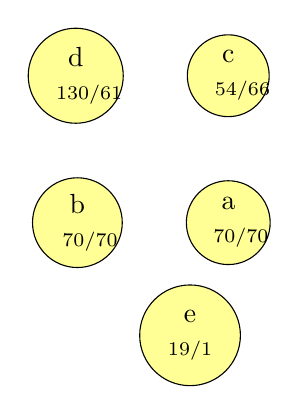
\begin{tikzpicture}[>=latex, auto,
node distance=0.8cm,
mynode/.style={
  circle,
  draw,
  fill=myyellow,
  text centered}
]
\mynode{0.50}{d}{130/61} %67
\mynode[right=of d]{0.34}{c}{54/66} %45
\mynode[below=of c]{0.38}{a}{70/70} %5
\mynode[left=of a]{0.38}{b}{70/70} %5
\mynode[below right=of b]{0.71}{e}{19/1} %95

\end{tikzpicture}
    \label{subfig:socialsupport}
    
  } \hspace{0.2 cm}
  \subfloat[{}]{
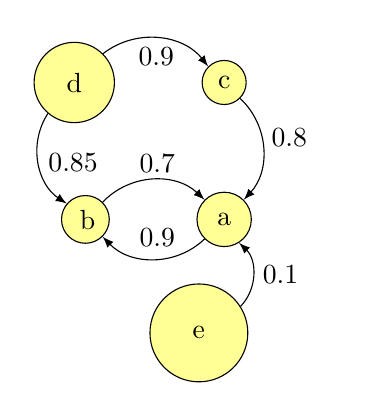
\begin{tikzpicture}[>=latex, auto,
node distance= 1.1 cm,
mynode/.style={
  circle,
  draw,
  fill=myyellow,
  text centered}
]
\mynode[]{0.67}{d}{}
\mynode[right=of d]{0.17}{c}{}
\mynode[below=of c]{0.34}{a}{} 
\mynode[left=of a]{0.14}{b}{} 
\mynode[below right=of b]{0.95}{e}{}
\draw [->] (d) to [bend left=45] node [pos=0.5, below, text width= 0.5cm] {0.9} (c);
\draw [->] (c) to [bend left=45] node [pos=0.4, right, text width=0.9cm]{0.8} (a);
\draw [->] (b) to [bend left=45] node [pos=0.7, above, text width=0.9cm]{0.7} (a);
\draw [->] (a) to [bend left=45] node [pos=0.3, above, text width=0.9cm]{0.9} (b);
\draw [->] (e) to [bend right=45] node [pos=0.5, right, text width=0.9cm]{0.1} (a);
\draw [->] (d) to [bend right=45] node [pos=0.5, right, text width=0.5cm]{0.85} (b);
 
\end{tikzpicture}
    \label{subfig:smodel}
  }  \hspace{-1 cm}
  \subfloat[{}]{
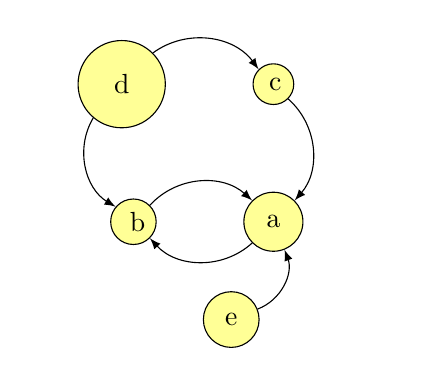
\begin{tikzpicture}[>=latex, auto,
node distance= 1.1 cm,
mynode/.style={
  circle,
  draw,
  fill=myyellow,
  text centered}
]
\mynode[]{0.77}{d}{}
\mynode[right=of d]{0.11}{c}{}
\mynode[below=of c]{0.41}{a}{} 
\mynode[left=of a]{0.09}{b}{} 
\mynode[below right=of b]{0.36}{e}{}
\draw [->] (d) to [bend left=45] node [pos=0.5, below, text width= 0.5cm] {} (c);
\draw [->] (c) to [bend left=45] node [pos=0.4, right, text width=0.9cm]{} (a);
\draw [->] (b) to [bend left=45] node [pos=0.7, above, text width=0.9cm]{} (a);
\draw [->] (a) to [bend left=45] node [pos=0.3, above, text width=0.9cm]{} (b);
\draw [->] (e) to [bend right=45] node [pos=0.5, right, text width=0.9cm]{} (a);
\draw [->] (d) to [bend right=45] node [pos=0.5, left, text width=0.5cm]{} (b);
\end{tikzpicture}

    \label{subfig:esafmodel}
  }
  
  \caption{ Framework with arguments scaled according to social support (a),  ESAF-model of the debate(b),  Model of the vector representation(c)}
 \label{fig:triple}
 
\end{figure}

\renewcommand{\tabcolsep}{0.3cm}
\begin{table}[ht]
  \caption{Model of the Social Abstract Argumentation Framework considering: a) social support only; b) ESAF; c) Vector representation;\\}
  \centering % used for centering table
\begin{tabular}{c c c c c} % centered columns (6 columns)
\hline\hline %inserts double horizontal lines
Argument &  Fig. a & Fig. b & Fig. c & \\ [0.7ex] % inserts table 
%heading
\hline % inserts single horizontal line
a & 0.50 & 0.35 & 0.41\\ % inserting body of the table
b & 0,50 & 0,14 & 0.09\\
c & 0,45 &  0,17 & 0.11 \\
d & 0,68 & 0,68 & 0.77 \\ 
e & 0,95 & 0,95 & 0.36 \\ [1ex] % [ex] adds vertical space
\hline %inserts single line
\end{tabular}
\label{table:figs} % is used to refer this table in the text
\end{table}



%As a recap, we semi-formally investigated the localised bi-dimensional approach for computing social support. Later, the result of this family of approaches (i.e. a bi-dimensional representation for each argument) will be utilised in a global manner by the system in order to associate each argument with the model evaluation.


At the first glance it seems as once the theoretic foundation is defined, this class of methodologies should not impose a computational overhead to the existing system; since computing the solutions will still be the problem of finding the fix-point of the model equations which is only preceded by a different method for computing social support. 
That being said, there are some significant pitfalls, sadly which oppose to the very nature of the incentives for using bi-dimensional representation:

\begin{enumerate}
\item Firstly, the choice of  a bi-dimensional representation makes sense the most for a particular context, where the domains of the vector components are not too restricted in their respective dimensions. So that potentially vector directions can point to every angle in the four quadrants of the cartesian space. In our example, we defined the system in a way that it assures the dimension regarding the size magnitude (x-axis) is alway non-negative. Assume the contrary; so that when an argument $a$ is attacked by a vector-force with a strong component in the x-axis, it may result to a negative $\tau(a_x)$ value. Users with bad intentions might exploit this notion in the following way: Suppose there is an argument $x$ that you want to defeat(see it's social support diminished). There are mainly two things that you will want to achieve: Firstly, trying to define as many attacks as you can. Followed by attempting to vote on these attacks as many times as possible. For our current topic of interest, it doesn't matter whether you can cast a high number of positive votes on the attack you defined. You are content as long as the total vote number increases. Because every vote casted on its attackers imposes a diminishing effect on $\tau(a_x)$, and since we allowed the component to obtain negative values, eventually the social support value, $\tau(a)$ might be decreased to a value point beyond recovery. On the other hand by restricting the domain of the component only to positive values, we are restricting the vector direction to two quadrants.

\item We have stated that the component in the y-axis of the vectors stand for the relative measure of positive and negative votes; and indeed utilized the original social support definition. In Social Argumentation Frameworks, we prohibit arguments obtaining negative social support values, and behaving as direct supporters to the arguments that they attack as it gives a way to the exploitation of the system. In order to strengthen an argument a user has defined, she may simply introduce a set of illogical arguments and attack relations from these argument to her initial argument. The basic idea is provoking the community and gathering as many negative votes as possible, and thus creating a set of \textit{artificial} supporters for the desired argument. Preventing this type of behavior was exactly our motivation in defining the component of the y-axis as non-negative as well. That being said, by restraining the domain values from acquiring negative values, we also restrict the direction of vectors to a single quadrant, mainly the first quadrant of the 2D cartesian-space.

\item Lastly, we should perhaps consider actions in 2D-space by their very nature. In very simple words, taking a step in the x-axis, and taking a step in y-axis are totally independent, orthogonal actions, whose results then can be interpreted in an aggregated way. However in our setting, even that they are processed in distinct way, both parameters that constitute the values of two dimensions are the same (i.e. $v^{+}$ and $v^{-}$ for a particular argument). Thus in our scenario, it does not seem as possible to claim the same orthogonal fundamentals with respect to definitions of our dimensions. 

\end{enumerate}


All in all,  this technical exercise has been beneficial in providing us one concrete method of model computation. Even if we decide on abandoning hybrid dimensions for good, a similar methodology may be adopted for other approaches such as the one depicted in Section 2.3. It also seems to do a good job in incorporating the magnitude of total number of votes in the final evaluation. 



%\bibliographystyle{plain}
%\bibliography{repMar14}

\end{document}